
%\section{Experiments}
\section{Experimental Evaluation}
\label{sec:experiments}


We evaluate REPMD and **** on a number of benchmark tasks. We first introduce the tasks used for testing REPMD and *****, then present the experiment results. Implementation details are provided in Appendix. 

\subsection{Tasks}
\label{subsec:tasks}
We test the performance of REPMD on a synthetic bandit problem and the algorithmic tasks from OpenAI gym library \citep{brockman2016openai}.  
%\subsubsection{Synthetic Bandit}

A simple synthetic multi-armed bandit problem is firstly used as an initial testbed.
%We develop a simple synthetic multi-armed bandit problem as an initial testbed. 
The problem has 10,000 distinct actions. The reward of each action $i$ is initialized by $r_i = s_i^{8}$, where $s_i$ is randomly sampled from a uniform distribution over $[0,1)$. We represent each action $i$ with a feature vector $\phi_i\in \mathbb{R}^{20}$, randomly sampled from a standard normal distribution. Let $\Phi=[\phi_1,\dots,\phi_{10,000}]$ denote the feature matrix. The policy is parameterized by a weight vector $\theta\in  \mathbb{R}^{20}$ and  defined by $\text{softmax}(\Phi^{\top}\theta)$. Note that we only learn the $\theta$ parameter, the features $\Phi$ are fixed during training. 

We further test our method on five algorithmic tasks from the OpenAI gym library, in rough order of difficulty: Copy, DuplicatedInput, RepeatCopy, Reverse, and ReversedAddition \citep{brockman2016openai}. In each problem, the agent operates on a tape of characters or digits. At each time step, the agent read one character or digit, and then decide to either move the read pointer one step in any direction of the tape, or write a character or digit to output. The total reward of each sampled trajectory is only observed at the end. The details of the tasks are provided in the Appendix.

Lastly, we test ***** using standard continuous-control benchmarks from OpenAI Gym utilizing the Mujoco environment \citep{brockman2016openai,todorov2012mujoco}, including Hopper, Walker2d, HalfCheetah, Ant and Humanoid. 

%\subsubsection{Algorithmic Tasks}

%We further test our method on five algorithmic tasks from the OpenAI gym library, in rough order of difficulty: Copy, DuplicatedInput, RepeatCopy, Reverse, and ReversedAddition \citep{brockman2016openai}. In each problem, the agent operates on a tape of characters or digits. At each time step, the agent read one character or digit, and then decide to either move the read pointer one step in any direction of the tape, or write a character or digit to output. The total reward of each sampled trajectory is only observed at the end. The goal for each task is:
%\begin{itemize}
%\item \textbf{Copy:} Copy a sequence of characters to output. 
%\item \textbf{DuplicatedInput:} Duplicate a sequence of characters.
%\item \textbf{RepeatCopy:} Copy a sequence of characters, reverse it, then forward the sequence again. 
%\item \textbf{Reverse:} Reverse a sequence of characters.
%\item \textbf{ReversedAddition:} Observe two numbers in base 3 in little-endian order on a $2\times n$ grid tape. The agent should add the two numbers together. 
%\end{itemize}


%\subsection{Baselines}
%
%We implement Policy Mirror Descent (PMD) to prove the effectiveness of the \emph{mean seeking} direction of KL divergence for policy optimization used in REPMD. Like in REPMD, we augment a separate tempreture parameter $\tau'\geq 0$ to the original objective function (\ref{max_expected_reward_plus_relative_entropy}) of PMD, which gives $\max_{\pi_\theta \in \Pi}{ \ep_{\rho \sim \pi_\theta}{  r(\rho)  - \tau \text{KL}(\pi_\theta \| \refPi) } + \tau'\cH(\pi_\theta) }$, to encourage further exploration of the policy. 
%
%For synthetic bandit problem, we compare REPMD against PMD, REINFORCE with entropy regularization (MENT) \cite{williams1992simple,williams1991function}, and under-appreciated reward exploration (UREX)\cite{nachum2017improving}. For algorithmic tasks, we compare REPMD against PMD and UREX. We omit MENT since it has been shown less effective than UREX in algorithmic tasks \cite{nachum2017improving}. 

\begin{figure*}[t]
\begin{center}
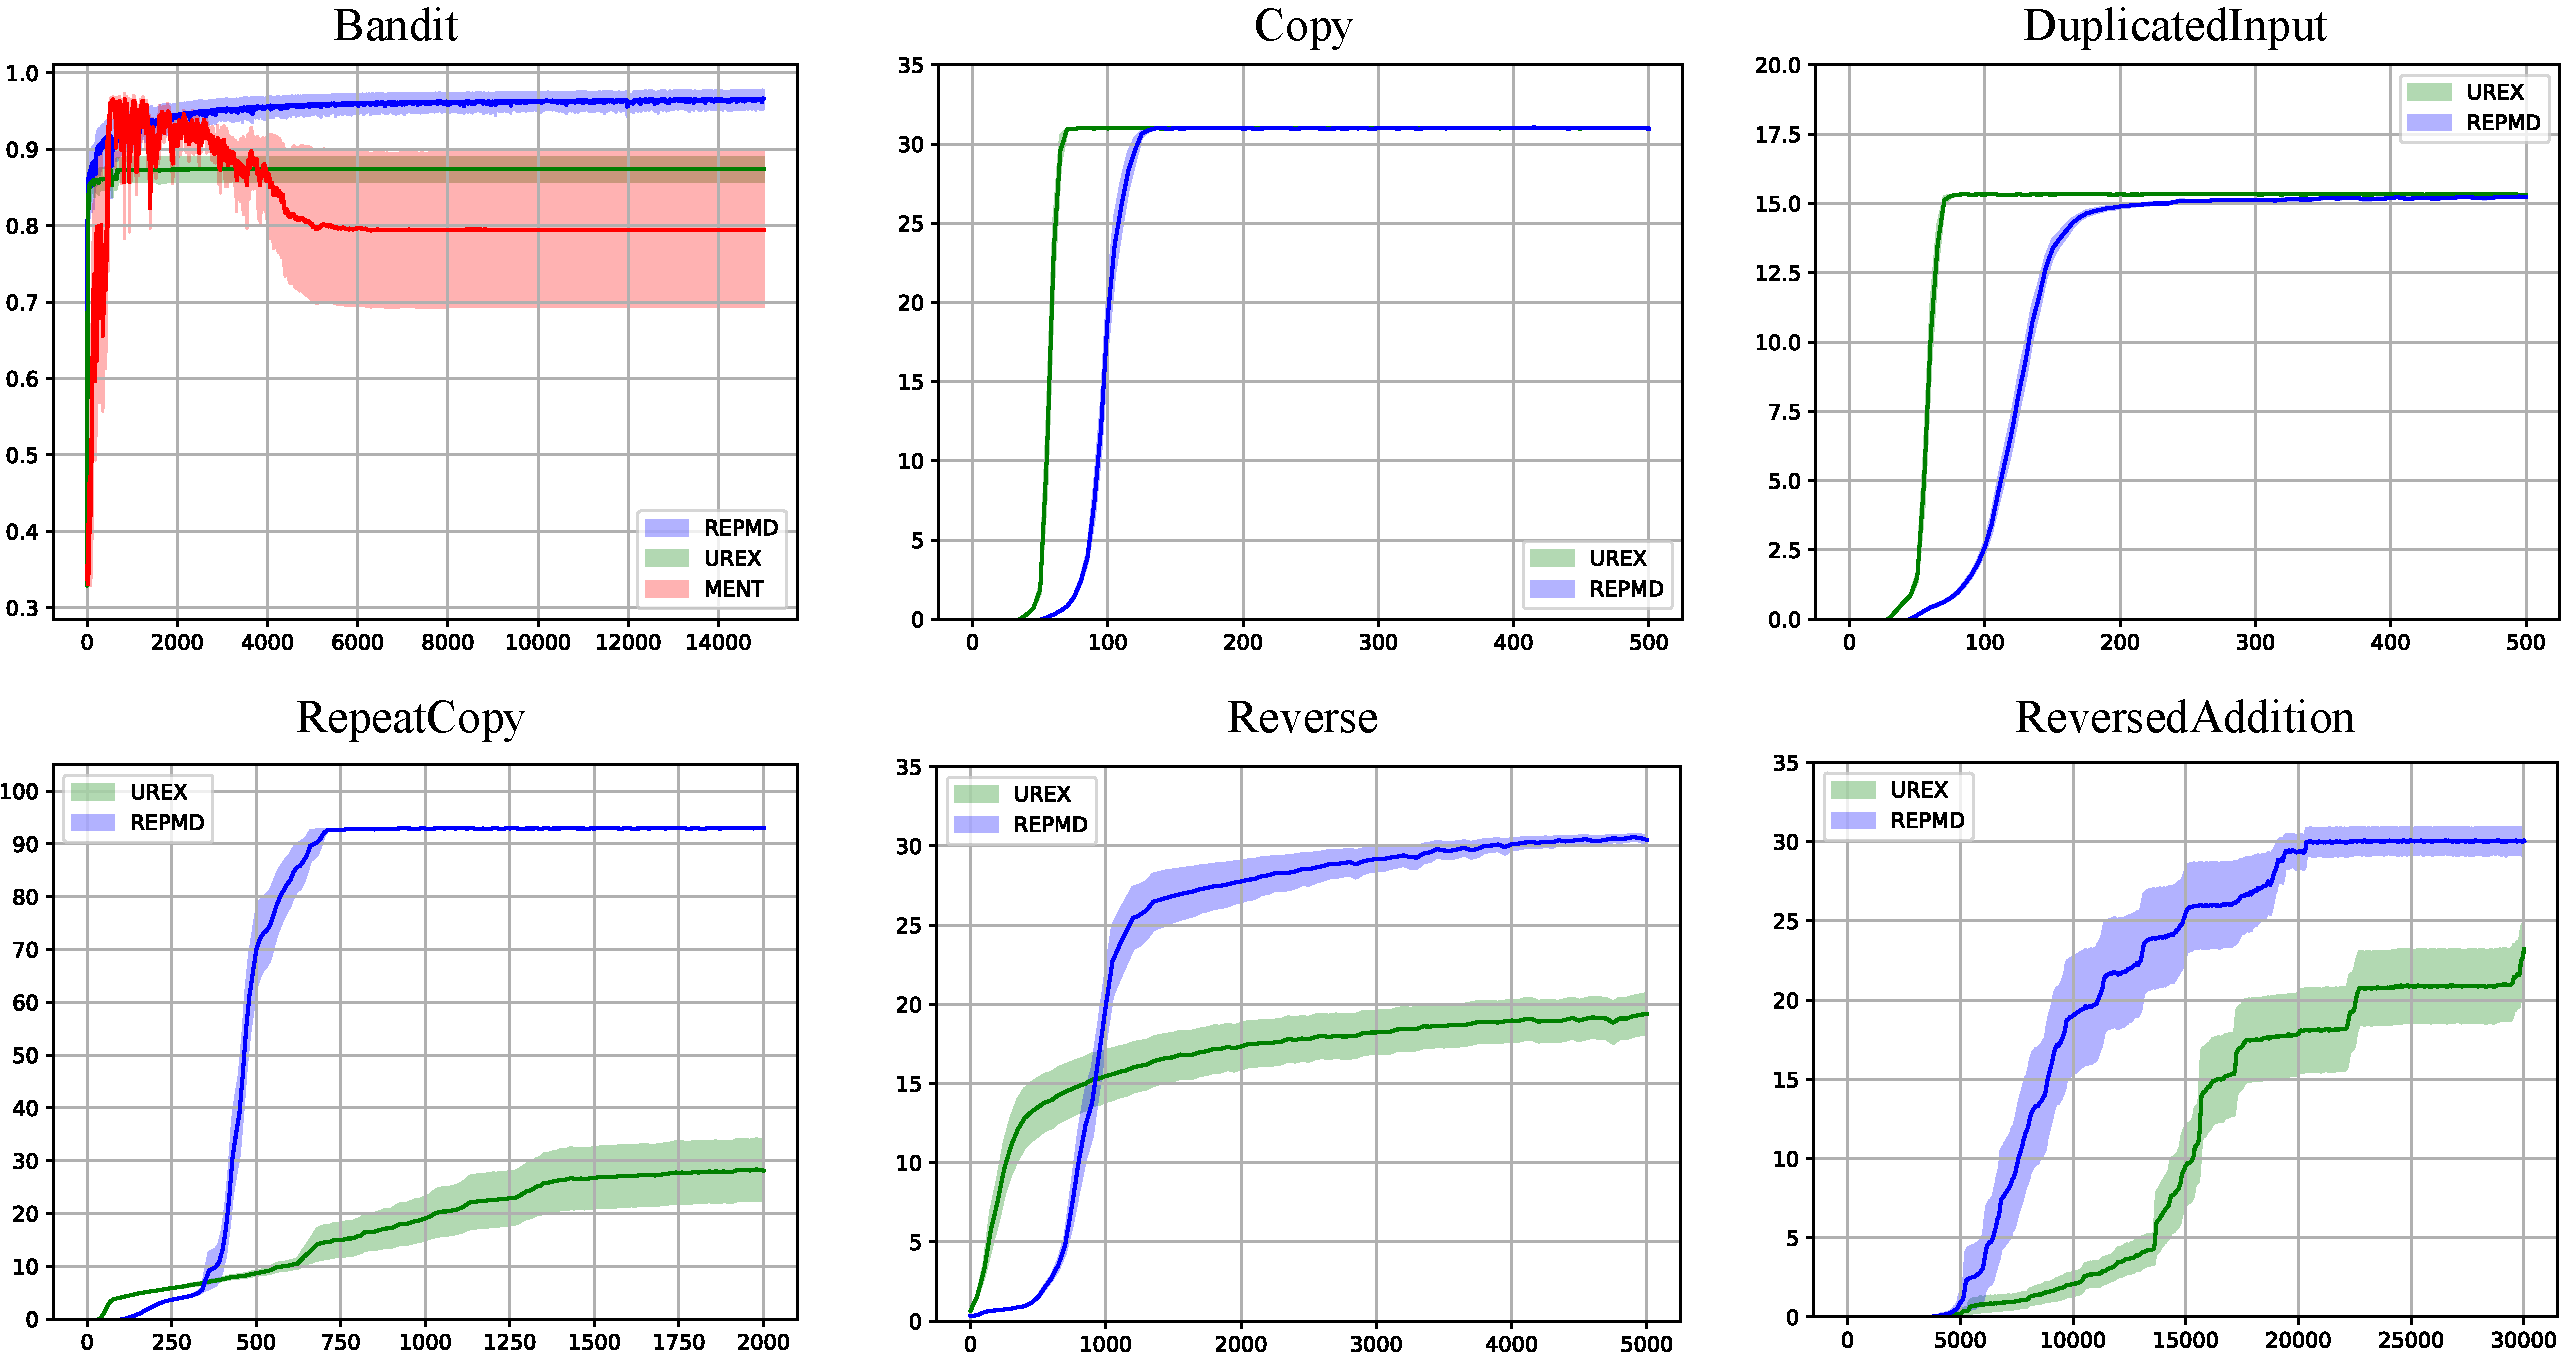
\includegraphics[width=0.85\linewidth]{./fig1.pdf}
\end{center}
\caption{
Results using the best hyper-parameters for each method: MENT (red), UREX (green), and REPMD (blue).
Plots show average reward with standard error during training. Synthetic bandit results averaged over 5 runs. Algorithmic task results averaged over 25 random training runs (5 runs $\times$ 5 random seeds for neural network initialization). X-axis is number of sampled trajectories. } 
\label{fig:results}
\end{figure*}

\subsection{Implementation Details}
\label{subsec:implementation}
For all of these algorithmic tasks, the policy is parameterized by a recurrent neural network with LSTM cells of hidden dimension 128 \citep{hochreiter1997long}. 

As shown in \cref{alg:repmd}, the policy is updated by performing KL divergence projection using stochastic gradient descent (SGD). In our experiments, the end condition of SGD is controlled by two parameters: $\epsilon > 0$ and $\text{F\_STEP}\in \{0,1 \}$. First, SGD halts if the change of the KL divergence is below or equal to $\epsilon$. Second, $\text{F\_STEP}$ decides the maximum number of SGD steps. If $\text{F\_STEP}=1$, the maximum number is $\sqrt{t}$ at iteration $t$; while if $\text{F\_STEP}=0$, there is no restriction on the maximum number of gradient steps, and stopping condition of SGD only depends on $\epsilon$.

For the synthetic bandit problem, we explore the following main hyper-parameters: learning rate $\eta \in \{0.1, 0.01, 0.001\}$; entropy regularizer of UREX and MENT $\tau\in \{1.0, 0.5, 0.1, 0.05\}$; relative entropy regularizer of REPMD $\tau\in \{1.0, 0.5, 0.1, 0.05\}$; $\epsilon\in \{0.01, 0.005, 0.001\}$ and $\text{F\_STEP}\in \{0,1\}$ for the stop condition of SGD in REPMD. The entropy regularizer $\tau'$ of REPMD is set to 0.

For the algorithmic tasks, $N$ distinct environments are used to generate samples. On each environment, $K$ random trajectories are sampled using the agent's policy to estimate gradient according to (\ref{eq:gradient_estimator}), which gives the batch size $N\times K$ in total. We apply the same batch training setting as in UREX \citep{nachum2017improving}, where $N=40$ and $K=10$. The following main hyper-parameters are explored: learning rate $\eta \in \{0.1, 0.01, 0.001\}$; relative entropy regularizer of REPMD $\tau\in \{1.0, 0.5, 0.1, 0.05\}$; entropy regularizer of REPMD $\tau'\in \{0, 0.01, 0.005, 0.001\}$; gradient clipped norm for training LSTM $c\in \{1, 10, 40, 100\}$; $\epsilon\in \{0.01, 0.005, 0.001\}$ and $\text{F\_STEP}\in \{0,1\}$ for the stopping condition of SGD in REPMD. Parameters of UREX are set according to the ones reported in \citet{nachum2017improving}. Implementations of all algorithm are based on the open source code by the author of UREX \footnote{\url{https://github.com/tensorflow/models/tree/master/research/pcl_rl}}.

\begin{figure*}[t]
\begin{minipage}{0.33\linewidth}
\centering
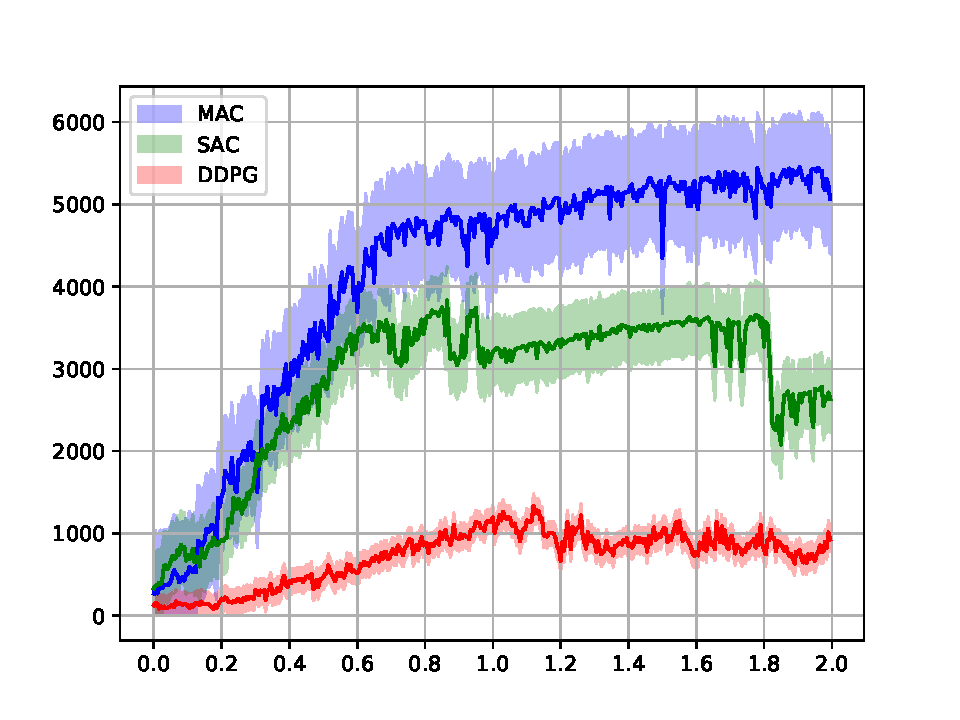
\includegraphics[width=2in]{./mujoco-results/Walker2d-v2-AVE.pdf}
%\caption{Error rate}
%\label{a}
\centerline{(a) Walker2d}
\end{minipage}%
\begin{minipage}{0.33\linewidth}
\centering
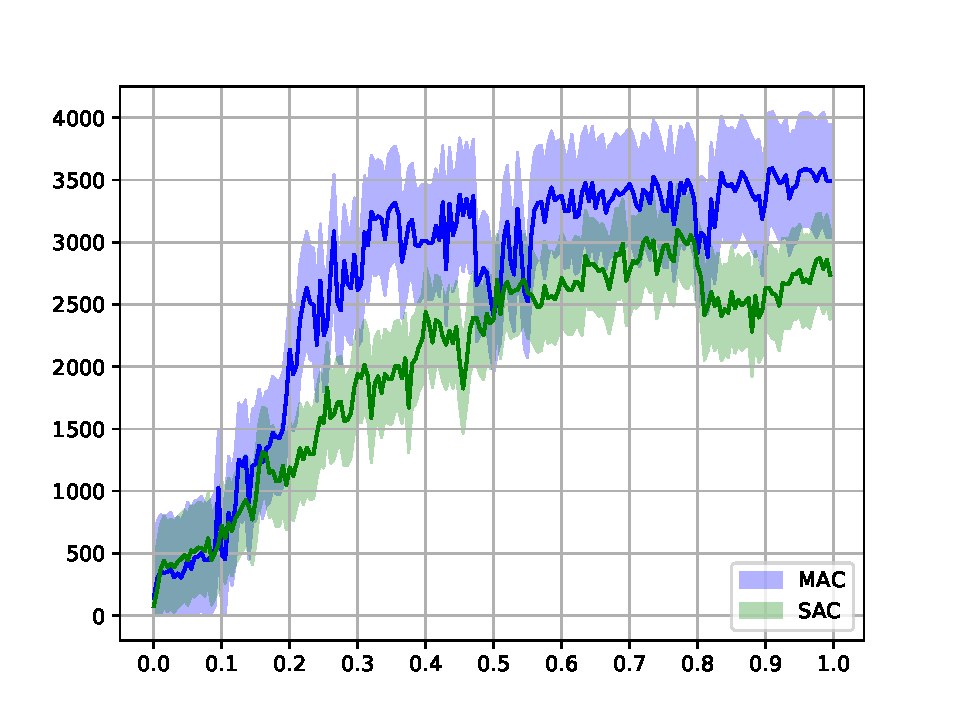
\includegraphics[width=2in]{./mujoco-results/Hopper-v2-AVE.pdf}
%\caption{Error rate}
%\label{a}
\centerline{(b) Hopper}
\end{minipage}%
\begin{minipage}{0.33\linewidth}
\centering
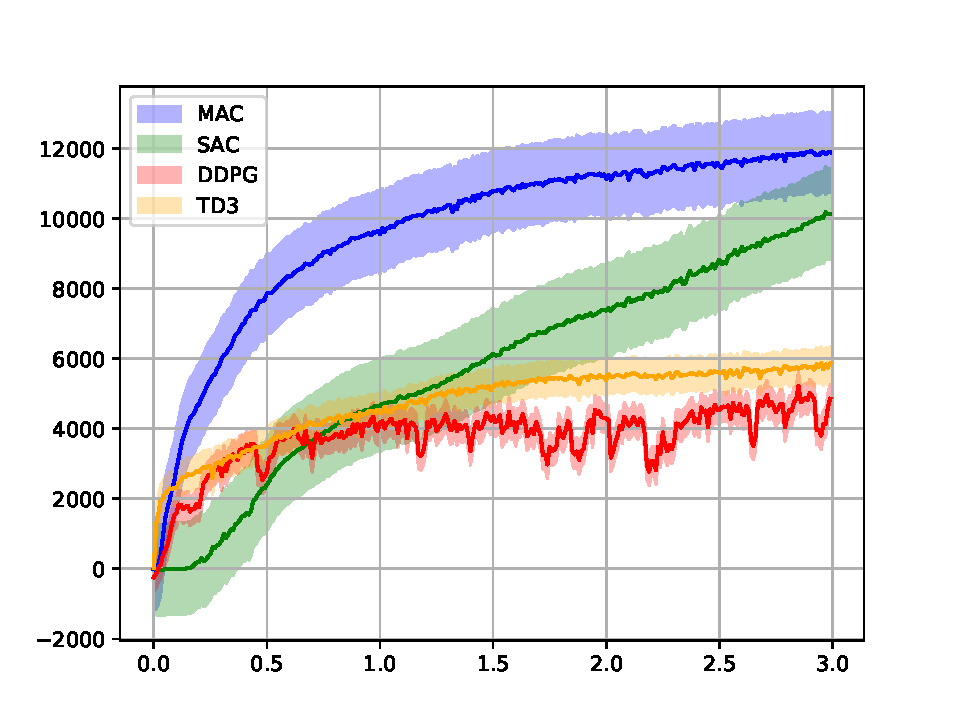
\includegraphics[width=2in]{./mujoco-results/HalfCheetah-v2-AVE.pdf}
%\caption{Error rate}
%\label{a}
\centerline{(c) HalfCheetah}
\end{minipage}%

\begin{minipage}{0.5\linewidth}
\raggedleft
%\centering
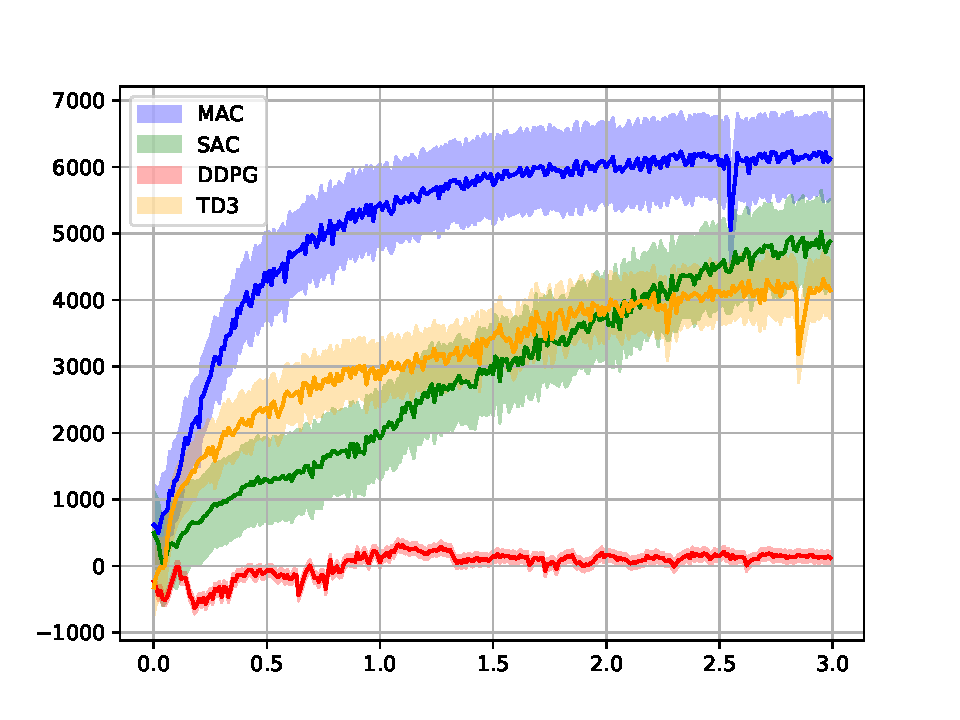
\includegraphics[width=2in]{./mujoco-results/Ant-v2-AVE.pdf}
%\caption{Error rate}
%\label{a}
\centerline{\ \ \ \ \ \ \ \ \ \ \ \ \ \ \       (e) Ant }
\end{minipage}%
\begin{minipage}{0.5\linewidth}
%\centering
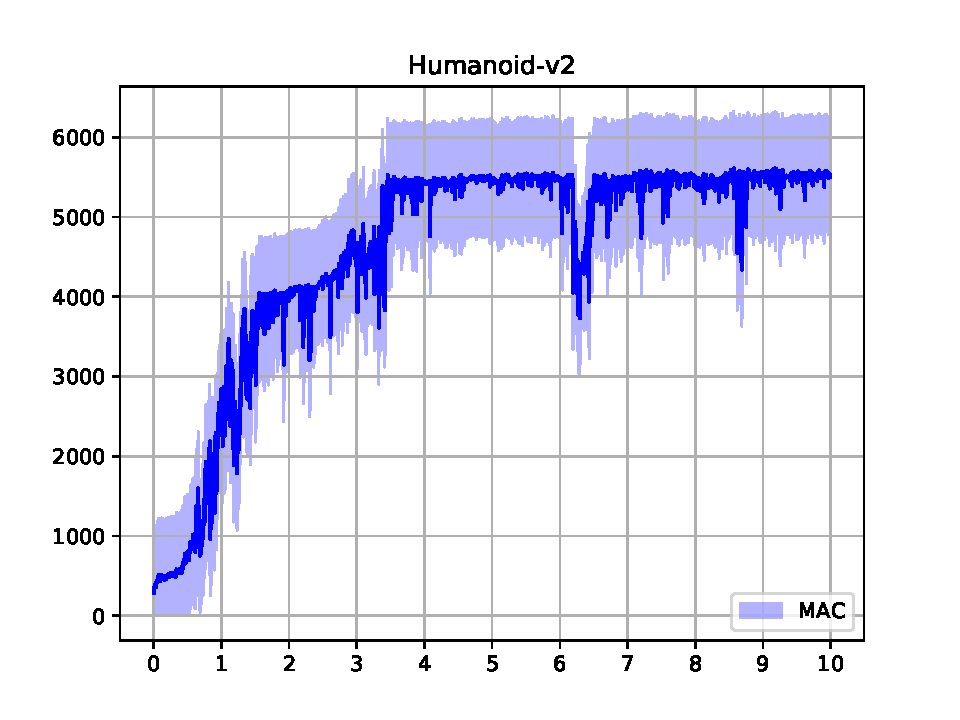
\includegraphics[width=2in]{./mujoco-results/Humanoid-v2-AVE.pdf}
%\caption{Error rate}
%\label{a}
\centerline{(f) Humanoid}
\end{minipage}%

\caption{Learning curves on continuous control benchmarks. }
\label{fig:result_mujoco}
\end{figure*}

\subsection{Comparative Evaluation}

\subsubsection{Experiments of REPMD}
For the synthetic bandit problem, we compare REPMD against REINFORCE with entropy regularization (MENT) \citep{williams1992simple} and under-appreciated reward exploration (UREX) \citep{nachum2017improving}. For the algorithmic tasks, we compare REPMD only against UREX, since UREX has been shown to outperform MENT in these cases \citep{nachum2017improving}. The results are reported in Figure (\ref{fig:results}). It is clear that REPMD substantially outperforms the competitors on all of these benchmark tasks. REPMD is able to consistently achieve the highest score and learn substantially faster than UREX. We also find the performance of UREX is very unstable. On the difficult tasks, including RepeatCopy, Reverse and ReversedAddition, UREX can only successfully find appropriate solutions a few times out of 5 runs for each random seed, which brings the overall scores down. This observation creates the gap between our presented results with the ones reported in the paper\footnote{The results reported in \citet{nachum2017improving} averages over 5 runs of random restart, while our results are averaged over 25 random training runs (5 runs $\times$ 5 random seed for neural network initialization). }. Note that the performance of REPMD is sill significantly better than UREX even compared with the results reported in \citet{nachum2017improving}. 

\subsubsection{Experiments of *****}

For continuous control tasks, we compare ***** to deep deterministic policy gradient (DDPG) \citep{}, an efficient off-policy deep
RL methods, twin delayed deep deterministic policy gradient algorithm (TD3), a recent extension to DDPG by applying the double Q-learning trick to address over-estimation problem when function approximation is used, and Soft-Actor-Critic (SAC), a recent state-of-the-art off-policy algorithm on a number of continuous control benchmarks. Figure \ref{} presents the total average return of evaluation rollouts during training of all algorithms on continuous control benchmarks. Results of each algorithm are averaged over five different instances with different random seeds. The solid curves corresponds to the mean and the shaded region to the standard errors over the five trials. The results show that...

%\begin{wrapfigure}{R}{0.5\textwidth}
%\label{fig:ablation}
%  \begin{center}
%    \includegraphics[width=0.5\textwidth]{Copy.png}
%  \end{center}
%  \caption{Hello, Bye!}
%\end{wrapfigure}

\subsection{Ablation Study}
\label{subsec:ablationstudy}
\piccaption[]{Ablation Study.\label{fig:ablation}}
\parpic[r]{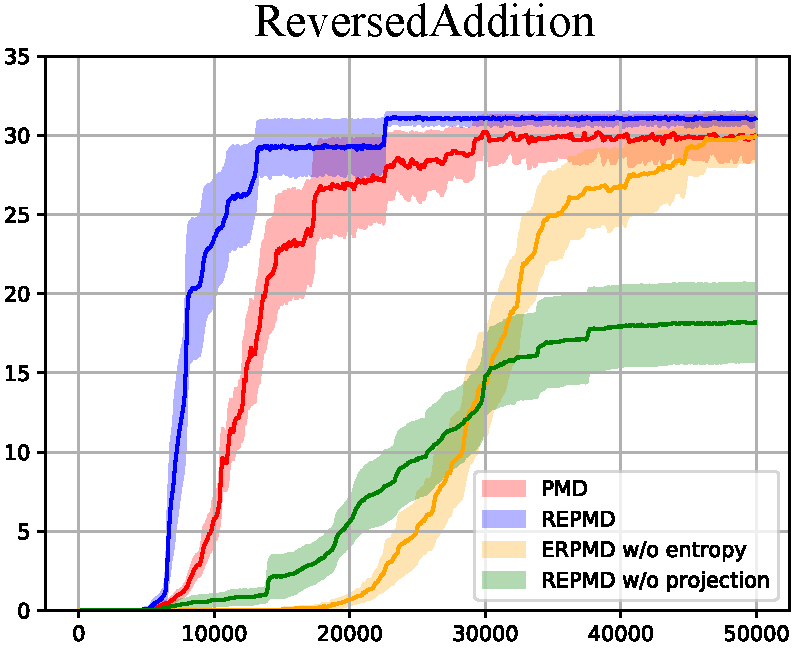
\includegraphics[width=0.35\linewidth]{ablation.pdf}}

\textbf{Importance of entropy regularizer.} The main difference between our objective \cref{eq:pmd} with the original MD is to add another entropy regularizer. We demonstrate the importance of this choice by presenting the results of REPMD with $\tau'=0$.

\textbf{Importance of KL divergence projection.} The main difference between REPMD and the UREX and MENT training methods is to use a projection step to optimize policy rather than performing a single gradient step. To show the importance of the projection step, we reimplement REPMD without projection, which only performs one step of gradient update at each iteration of training. 

\textbf{Importance of direction of KL divergence.} We implemented Policy Mirror Descent (PMD) as another baseline to prove the effectiveness of using the \emph{mean seeking} direction of KL divergence for policy optimization. Like in REPMD, we add a separate tempreture parameter $\tau'\geq 0$ to the original objective function (\ref{eq:max_expected_reward_plus_relative_entropy}) of PMD to encourage further exploration of the policy, which gives $\argmax_{\pi_\theta \in \Pi}{ \ep_{\rho \sim \pi_\theta}{  r(\rho)  - \tau \text{KL}(\pi_\theta \| \refPi) } + \tau'\cH(\pi_\theta) }$.

Results on ReversedAddition are reported in Figure (\ref{fig:ablation}). It clearly shows that optimizing policy by performing the \emph{mean seeking} KL divergence projection is very important as suggested in REPMD. 
